% APJ Reference: http://aas.org/journals/authors/common_instruct#_Toc2

\documentclass[iop]{emulateapj}
% \documentclass[12pt,preprint]{aastex}


% Define the sun symbol for use with solar mass
% \newcommand{\Sun}{\odot}
\newcommand{\vect}[1]{\boldsymbol{#1}}
% \usepackage{amssymb}
%\usepackage{xfrac}
% \usepackage{amsmath}
\usepackage{natbib}
\usepackage{footnote}
% \usepackage{multirow}
% \usepackage{array}
% \usepackage[lofdepth,lotdepth]{subfig}
\usepackage{todonotes}

\newcommand{\TODO}[1]{\todo[inline]{#1}}
\usepackage{float}

% \newcolumntype{x}[1]{%
% >{\centering\hspace{0pt}}p{#1}}%


\bibliographystyle{apj}

\shortauthors{Brenner}
\shorttitle{Characterizing stellar phenomena with fractals and multifractals}

%--------------------
%	Begin document
%--------------------
\begin{document}
%
\title{Fractal and Multifractal Analysis as Tools to Characterize Supernovae and Molecular Clouds: \\
subtitle}
%
\author{Samuel Brenner\altaffilmark{1}}
\email{samuel.e.brenner@gmail.com}
%\author{Tomasz Plewa\altaffilmark{1}}
%\email{tplewa@fsu.edu}
%
%\author{Andrzej Odrzwolek\altaffilmark{2}}
%\email{andrzej's email}
%
\altaffiltext{1}{Young Scholars Program, Florida State University}
%
%
%
%--------------------
%	Begin Abstract
%--------------------
\begin{abstract}
\end{abstract}
%
%
%
%--------------------
%	Begin keywords
%--------------------
\keywords{supernovae, fractals, multifractals}
%
%
%
%--------------------
%	Begin Body
%--------------------

\section{Introduction}
Many physical phenomena cannot be characterized by the idealizations of Euclidean geometry alone; they exhibit ``roughness''. That is, they have a detailed structure at any arbitrarily small size scale \citep{Falconer2003}. The development of \textit{fractal geometry} allows a mathematical treatment of the ``roughness'' inherent in the non-idealized phenomena of the real world. Multifractal analysis permits us to examine how those fractal characteristics themselves change with scale; in fact, they may even be fractal themselves. In this paper, we detail the application of fractal geometry to flame fronts in white dwarfs and then analyze the multifractal characteristics of star-forming molecular clouds.

\subsection{Fractal analysis of type Ia supernova flame fronts}
The accepted model for a type Ia supernova is a white dwarf that accumulates mass from a binary companion until it reaches a mass so large that the compression of the heavier elements in the core causes them to ignite and fuse, releasing more energy in the process. This deflagration results in a flame front that spreads rapidly throughout the star and causes the visible effects of supernova.

The surface of the expanding flame front can be dramatically affected by multiple types of turbulence. \cite{Landau1959} showed that the flame surface is subject to Landau-Darrieus instability in which the front is convoluted due to thermal expansion across the flame front. It is also widely established (see \cite{Kull1991}) that Rayleigh-Taylor instability, in which a denser fluid pushes through a less-dense one under the influence of a gravitational field, can contort the deflagration front in a supernova. 

These wrinkles on the surface of the flame front increase the front's effective surface area, and because the flame speed is proportional to the flame's surface area, the convolution of the surface can influence the rate at which the flame consumes the star. Thus, characterizing the shape of the flame front plays a crucial part in characterizing the supernova explosion process as a whole.\todo[inline]{Add new picture with darkened contour!}

\begin{figure}[t]
\begin{center}
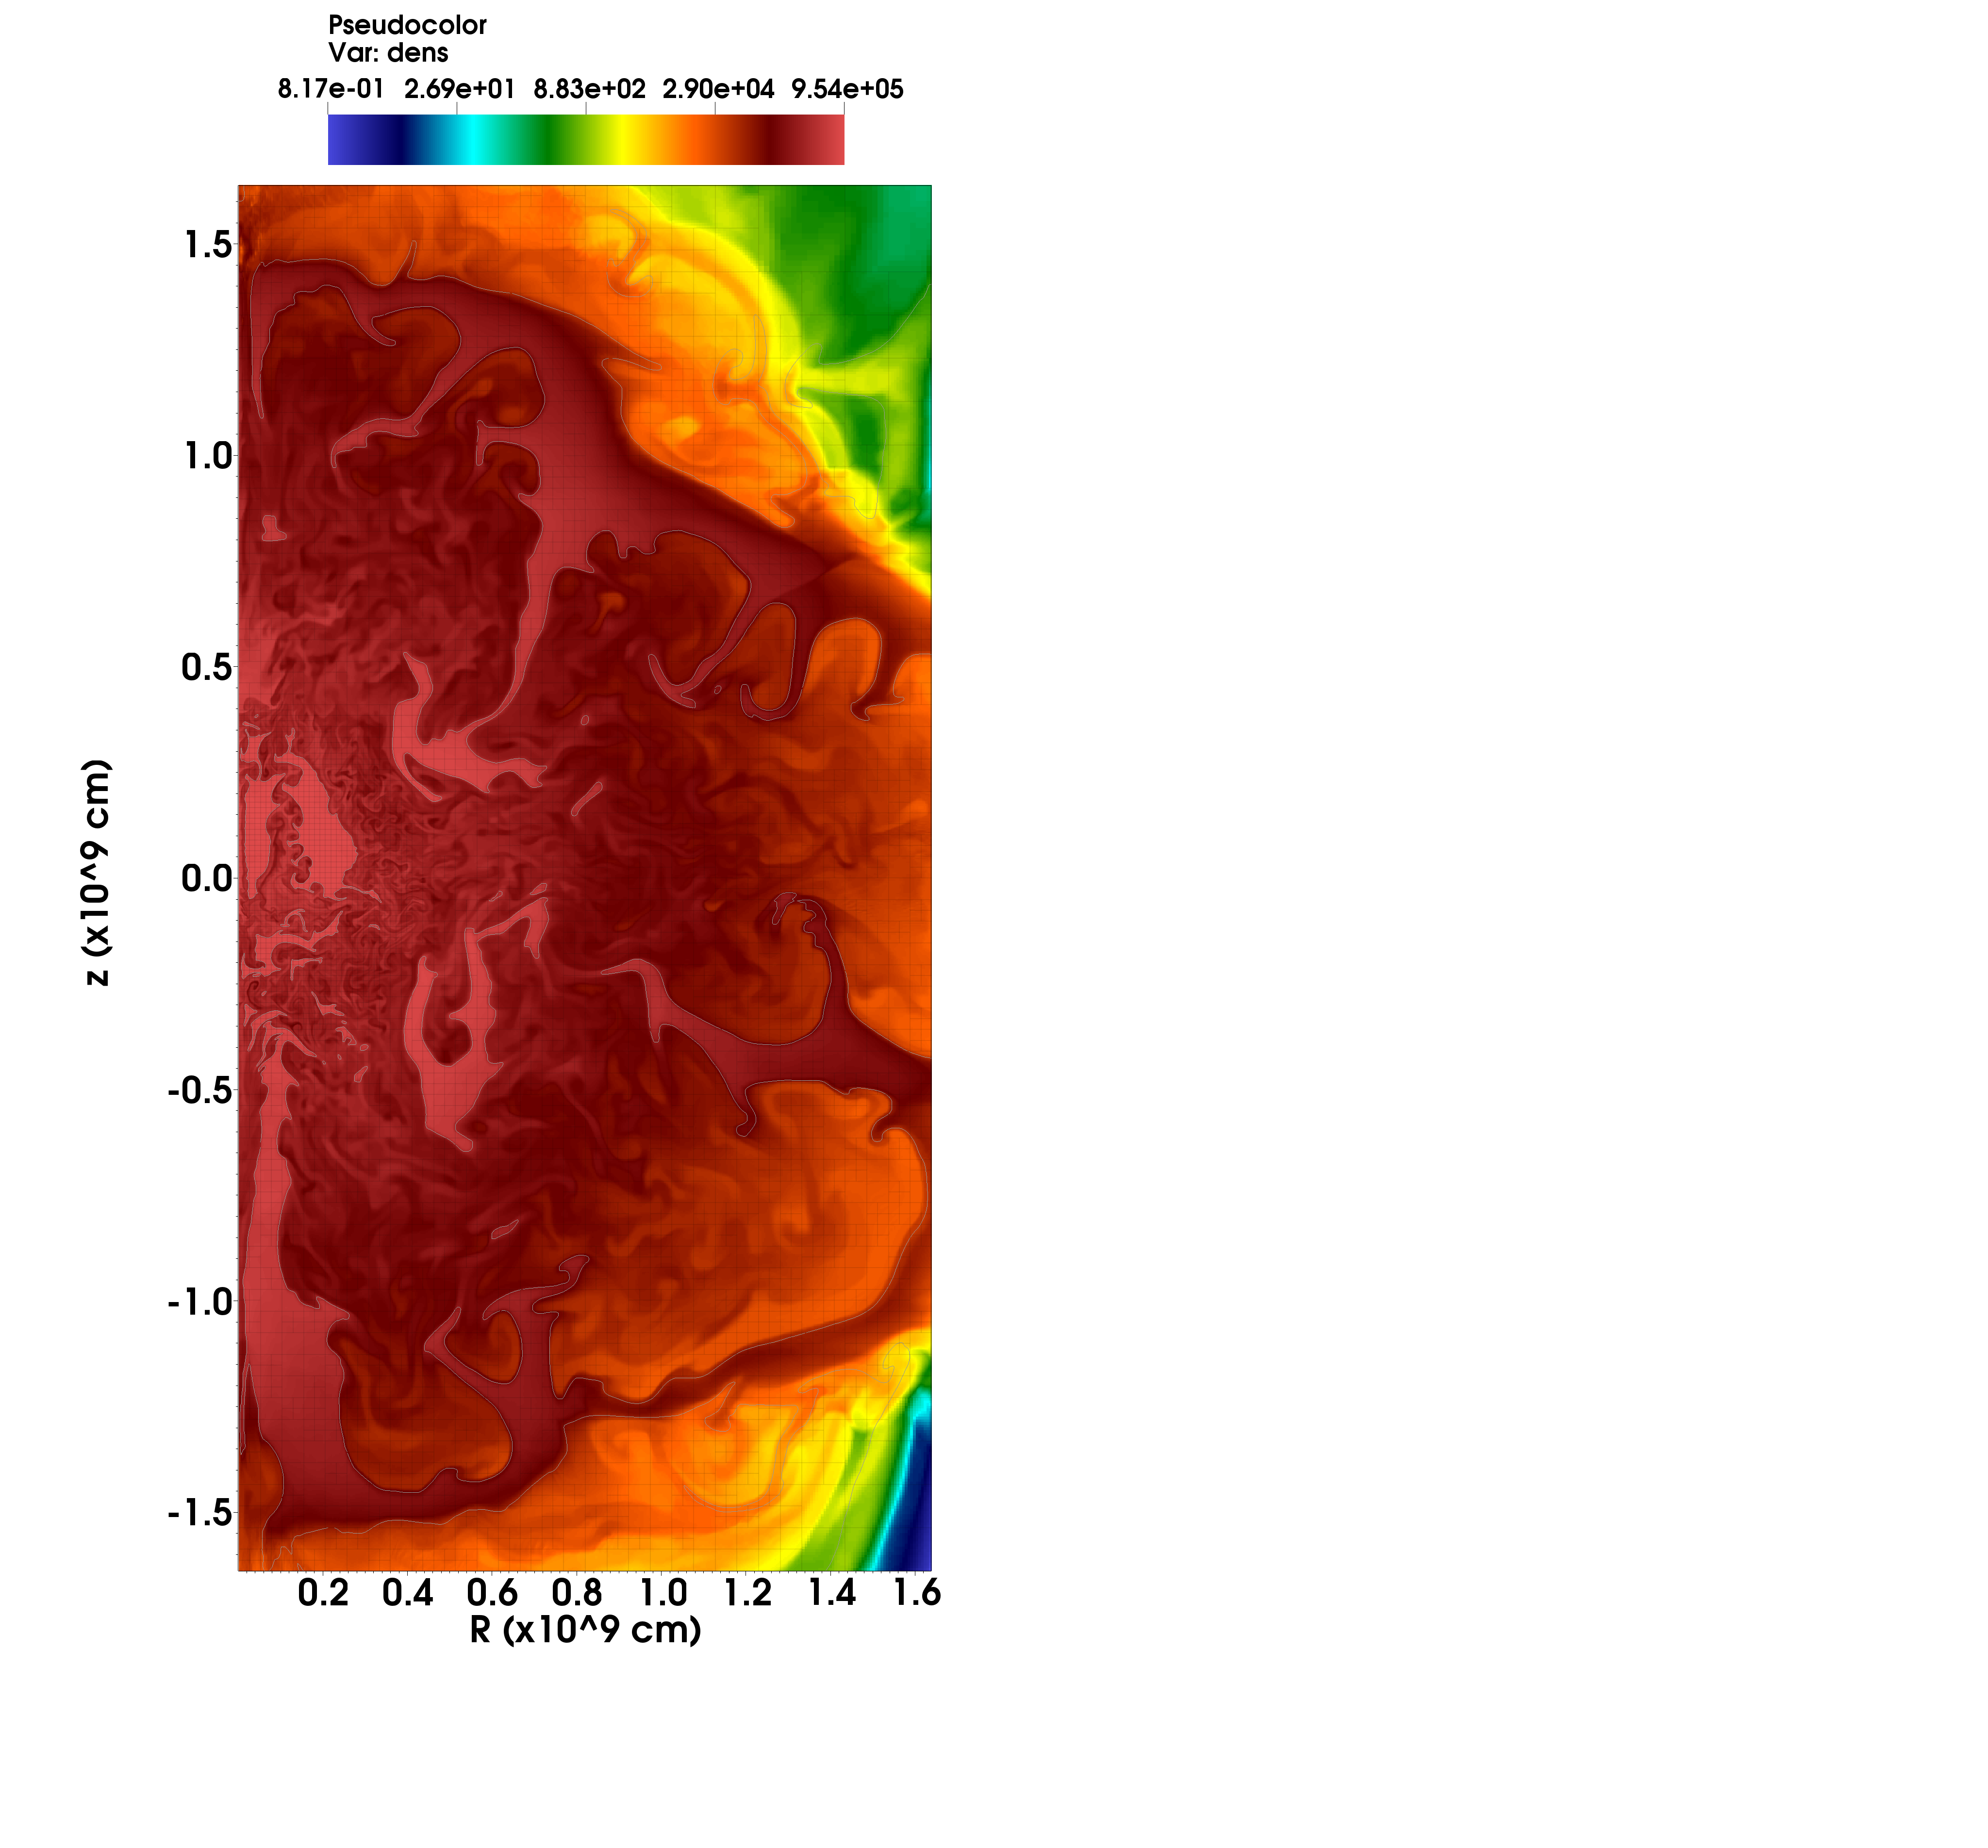
\includegraphics[width=0.45\textwidth,clip=true]{Graphics/n7d1r10t15b0002.png}
\caption{Flame front contour highlighted in simulation of Type Ia supernova. False color indicates density in $\mathrm{g/cm^3}$.
\label{f:flamefrontwithcontour}}
\end{center}
\end{figure} 

These wrinkles on the surface of a turbulent front can be viewed within the framework of fractal geometry, as was proposed by \cite{Mandelbrot1975} and further developed by \cite{Timmes1994}. Furthermore, \cite{Timmes1994} showed that the final effective speed of the flame front is a function of its density.

In \textsection \ref{FractalMethods}, a method is implemented to perform fractal analysis of a supernova flame front. The results are discussed in \textsection \ref{FractalResults}, and the implications of the calculated fractal dimension are discussed in \textsection \ref{FractalDiscussion}.

%%%%%%%%%%%%%%%%%%%%%%%%%%%%%%%%%%%%%%%%%%%%%
% Begin copy-pasting--needs editing			%
%%%%%%%%%%%%%%%%%%%%%%%%%%%%%%%%%%%%%%%%%%%%%

\subsection{Mutlfractal analysis of dense molecular clouds}
Clouds of gas often form in the interstellar medium (ISM), and turbulence like that caused by stellar winds can form structures which under gravitational pressure then coalesce into filaments. The densest parts of these filaments are protostars that begin to undergo fusion and merge to form evolved star systems. The structure of the system at any time can be quantified by the spectrum of multifractal dimensions, which indicates the density of substructures with a given density. Thus we can quantitatively indicate how uniformly filament-, sheet-, or space-like any structure is. Figures 2-4 depict the evolution of one of these molecular clouds.

\begin{figure*}[ht]
\begin{center}
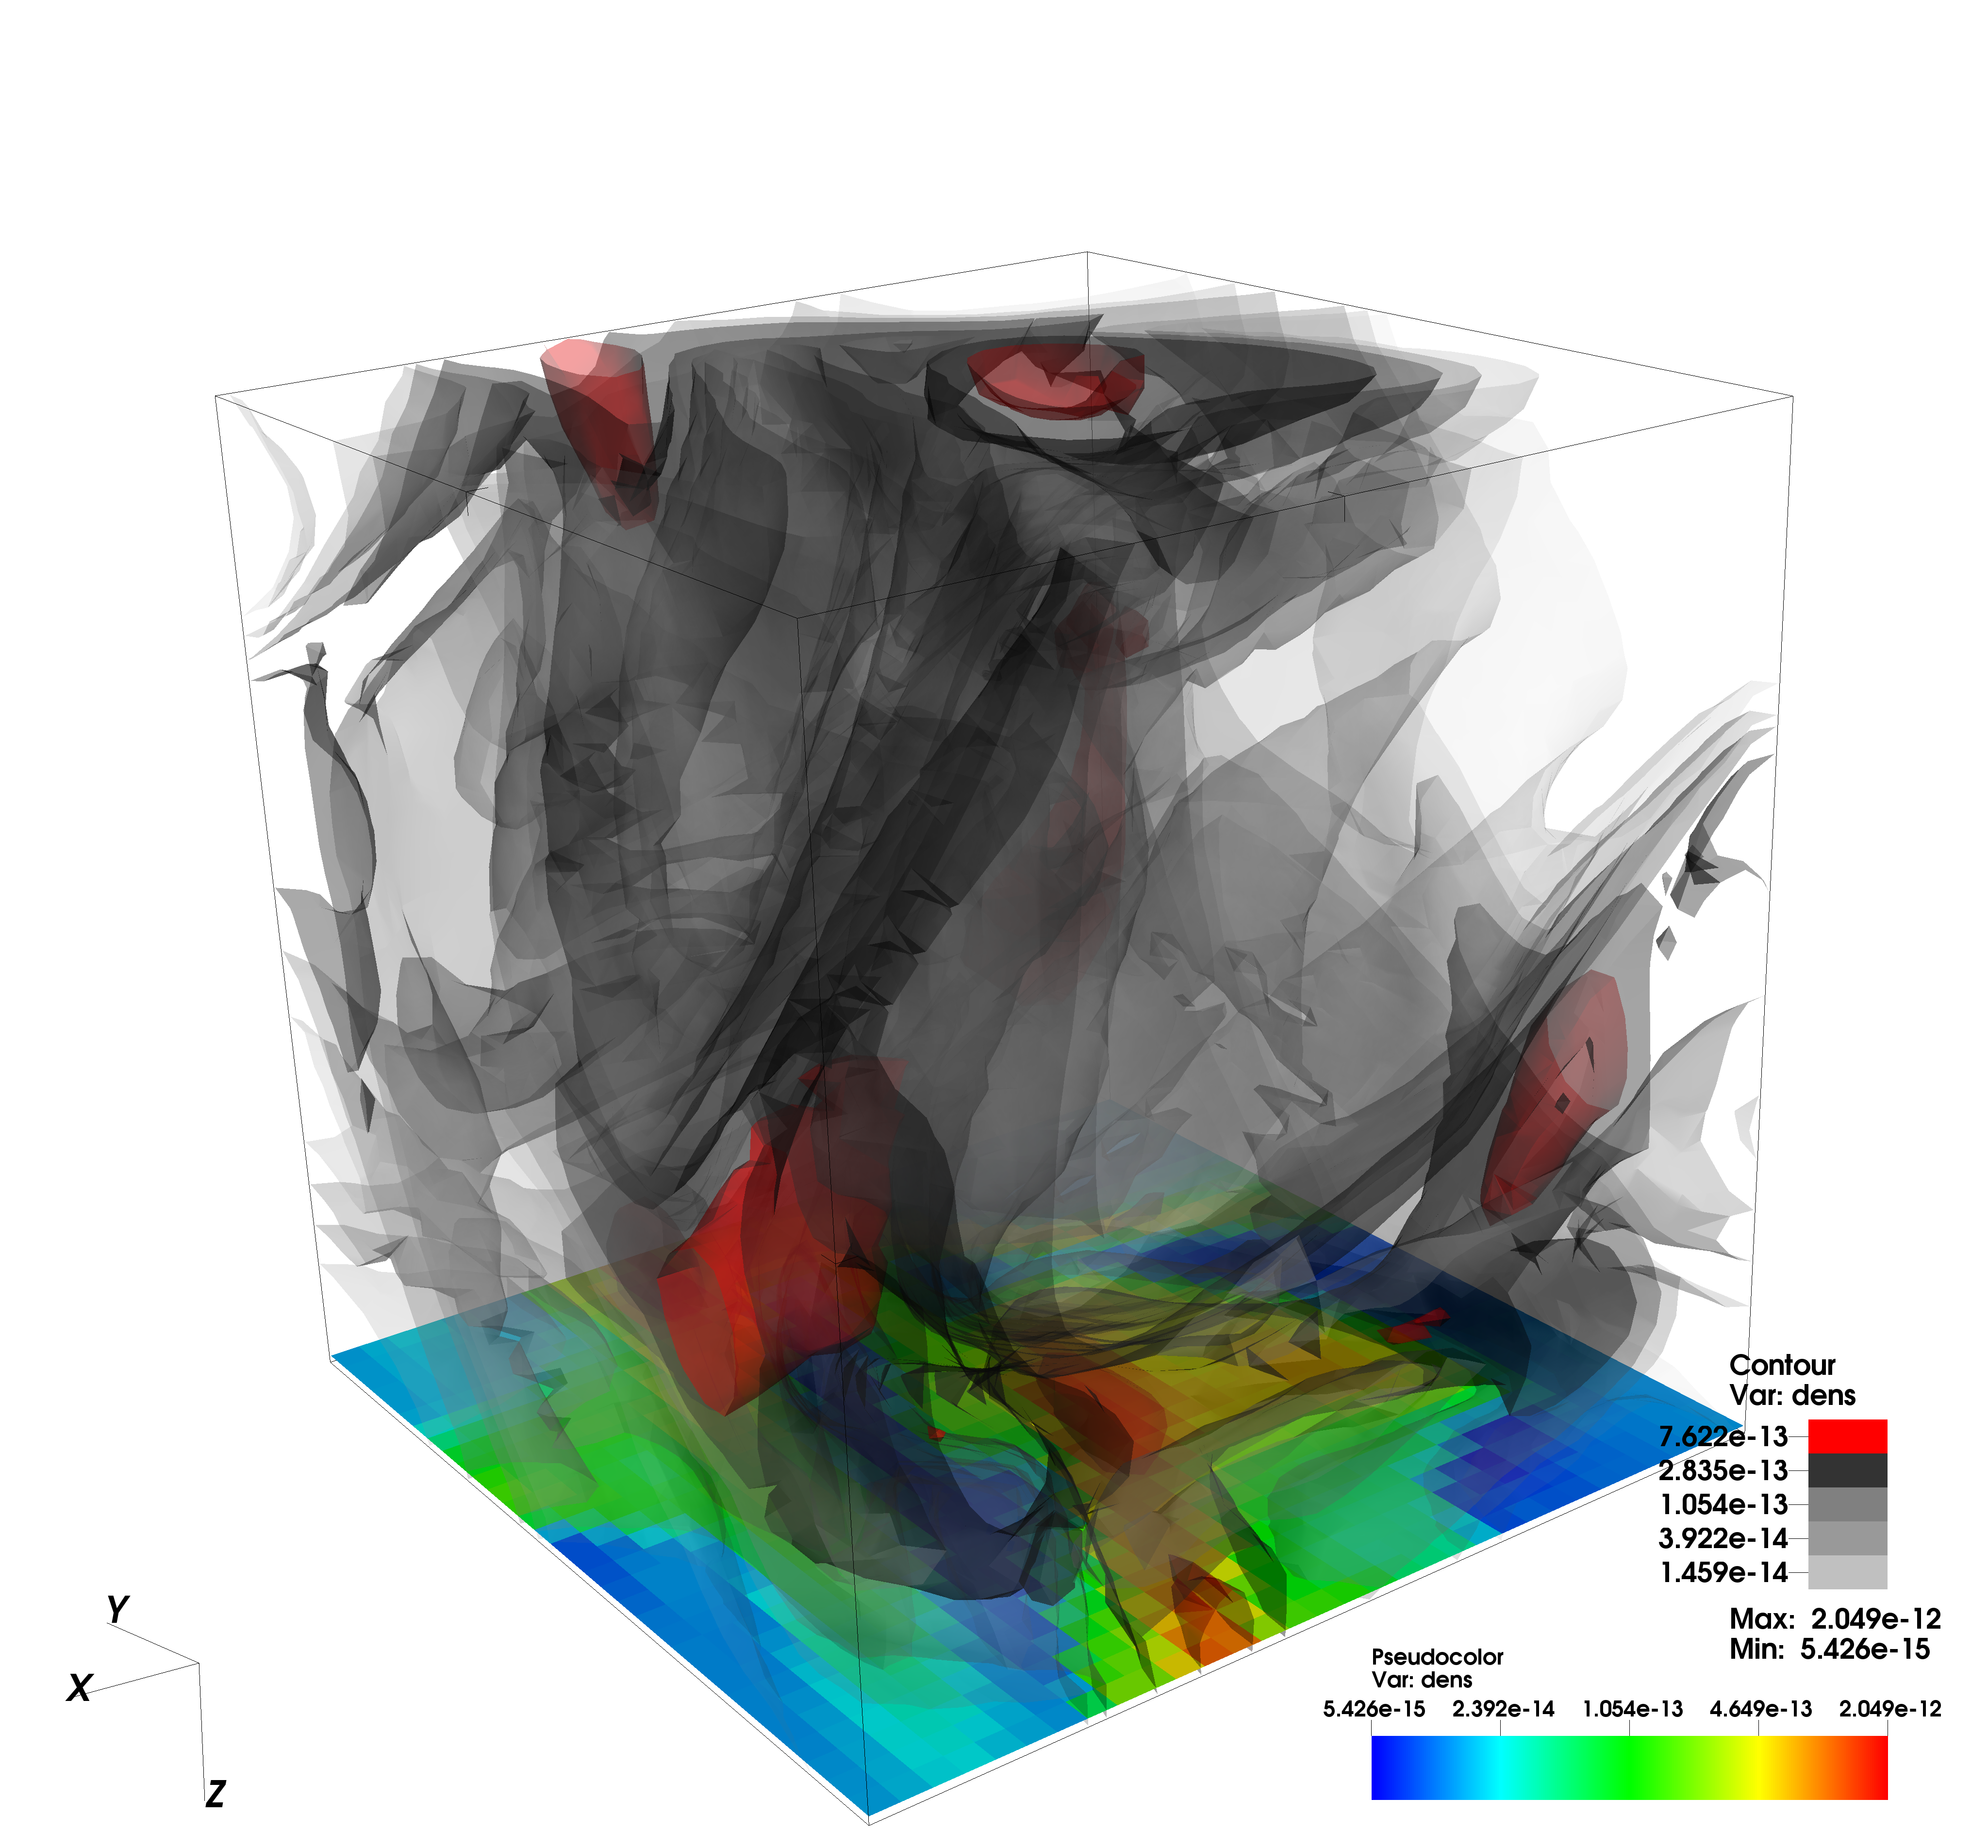
\includegraphics[height=5.5cm,clip=true]{Graphics/bbb_0375_dens_contour_00500000.png}%
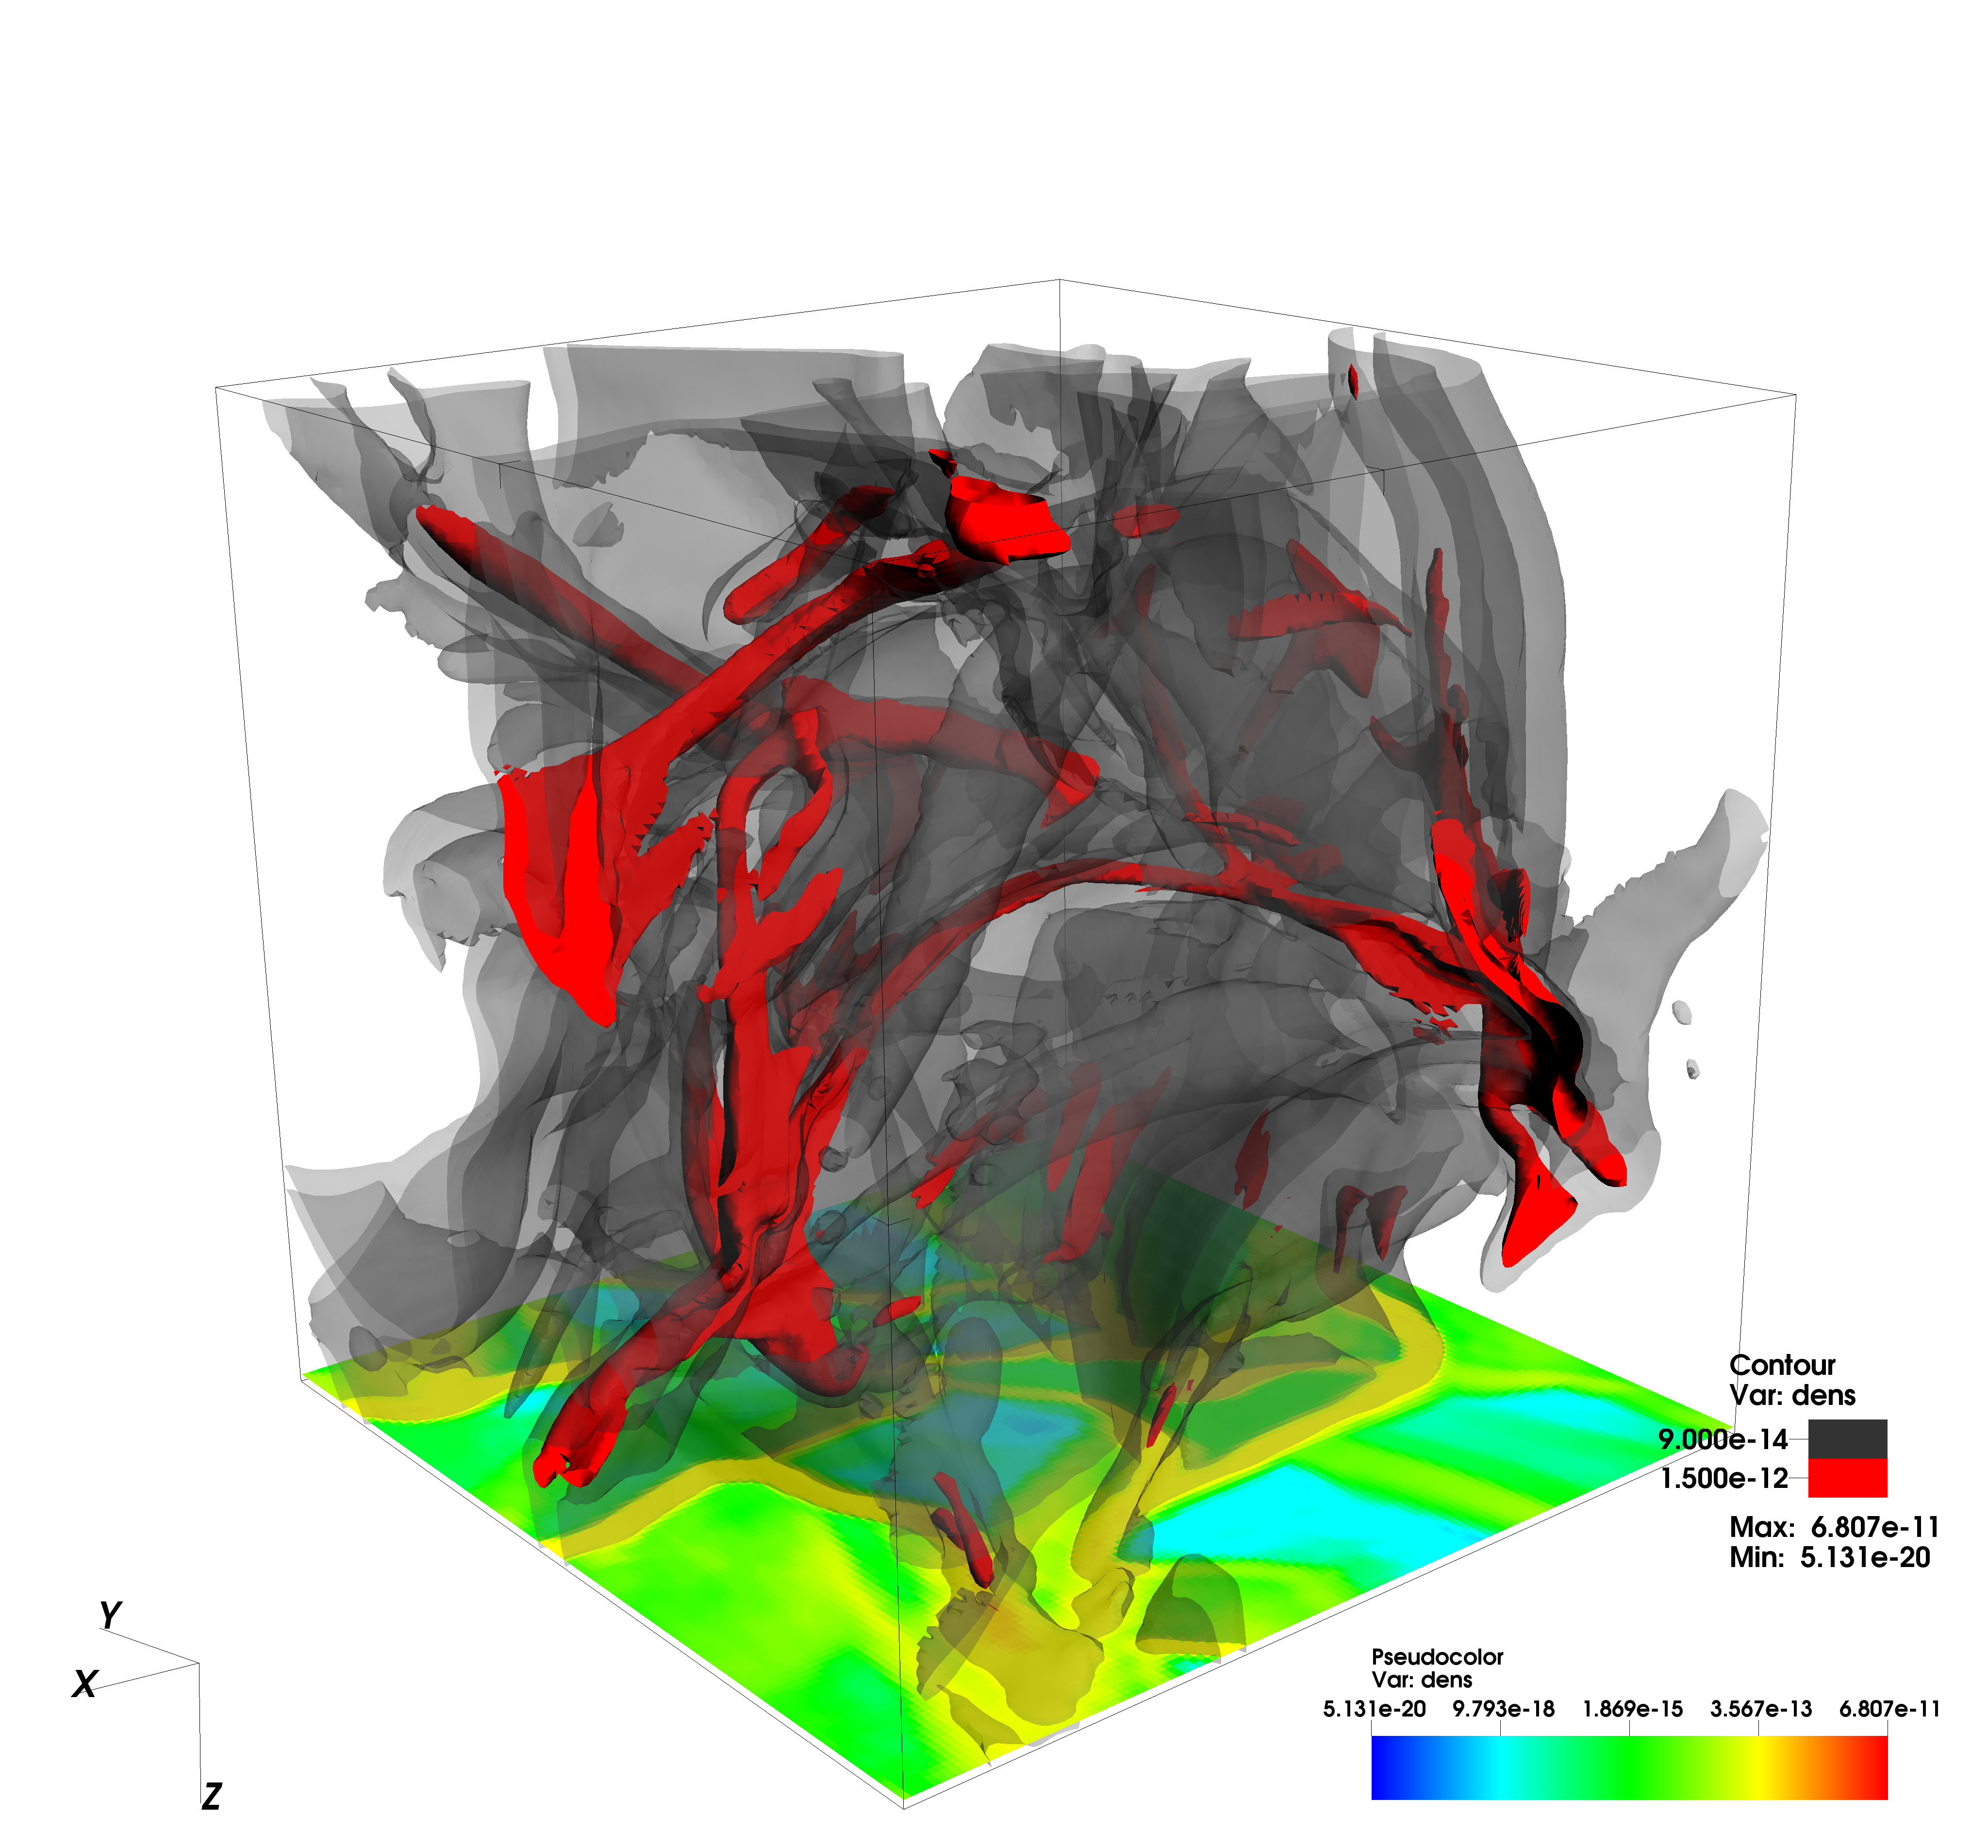
\includegraphics[height=5.5cm,clip=true]{Graphics/bbb_0375_dens_contour_0200_0002.png}%
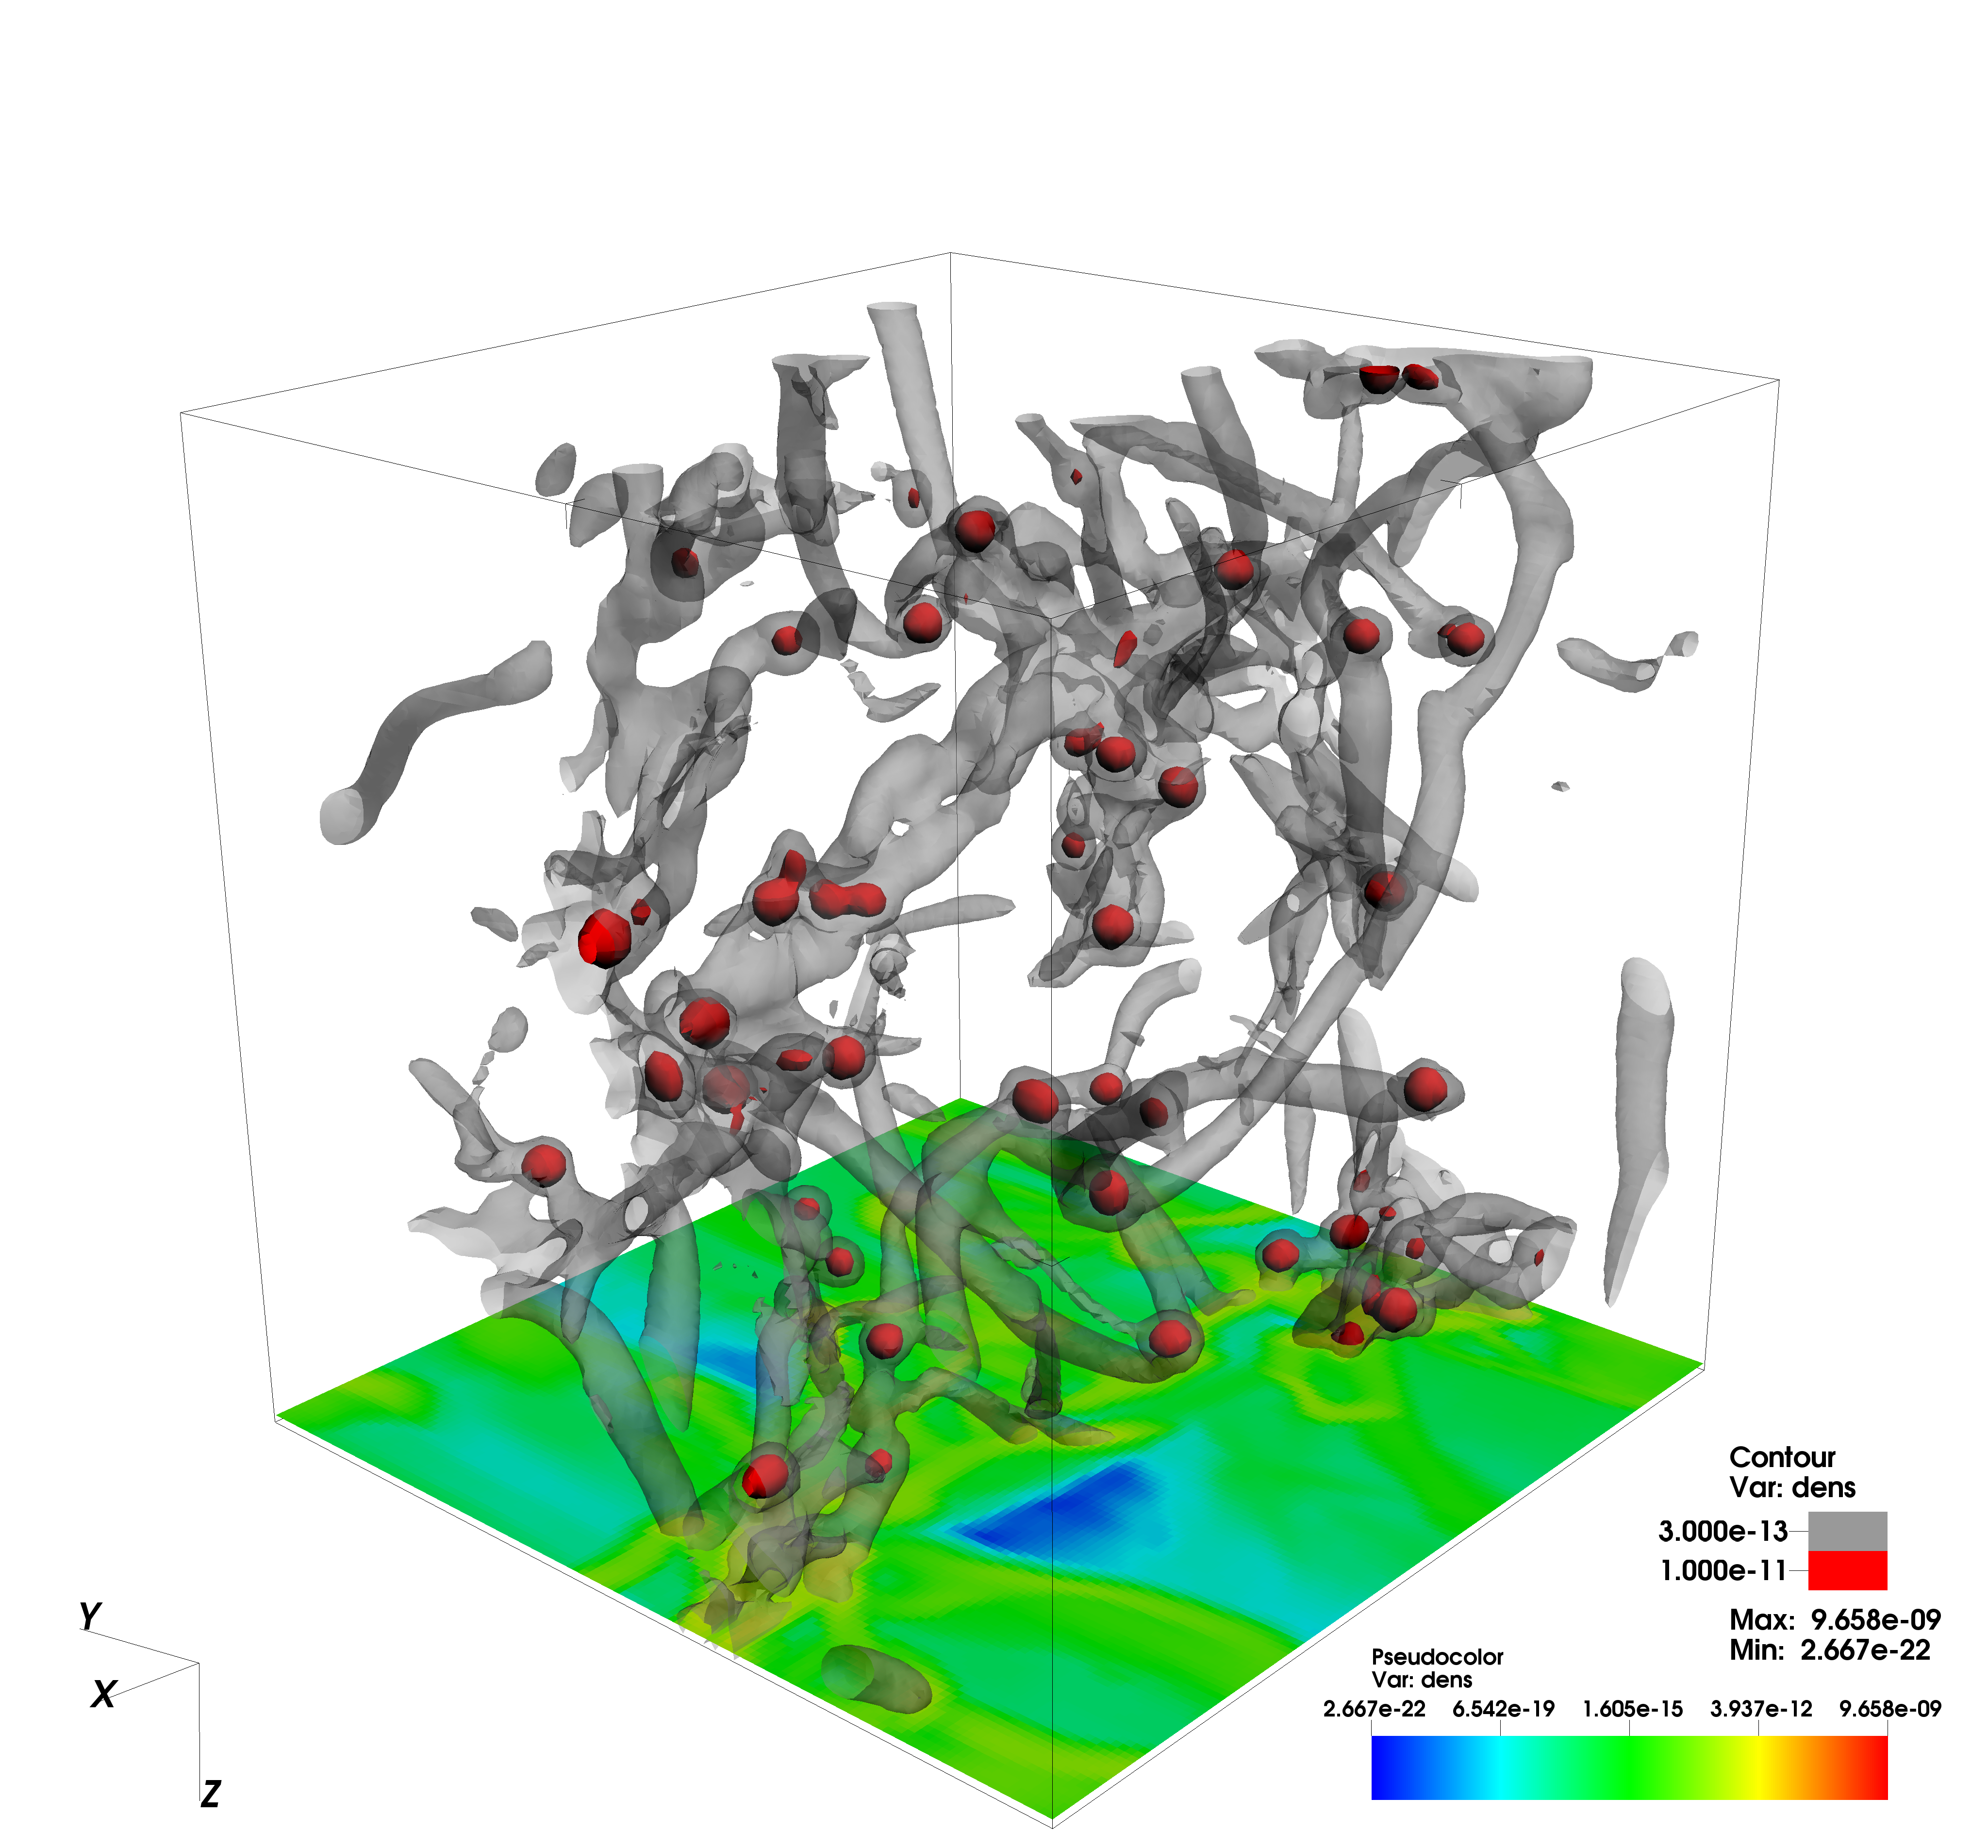
\includegraphics[height=5.5cm,clip=true]{Graphics/bbb_0375_dens_contour0000.png}
\end{center}
\caption{Evolution of a star-forming molecular cloud over time. The leftmost panel shows the density contour just after perturbation, with sheet-like structures most prominent. The middle panel shows the collapse of those sheets into filaments in the densest (red) regions. The rightmost panel shows a near-complete transition to filaments, and the densest (red) regions indicate the position of protostars.}
\label{f:cloudevolution}
\end{figure*}

\section{Methods}\label{Methods}
{\Large Write anything here?}

\subsection{Fractal analysis methods}\label{FractalMethods}
In order to estimate the fractal dimension of flame we implemented a box-counting algorithm. The box-counting dimension $\mathrm{dim}$ is given by

where N is the number of boxes containing the figure.  To implement this algorithm, different levels of coarse-graining were applied, and trilinear interpolation was performed to determine the location of the flame front within the coarse mesh. For each level of coarse-graining, $\log{N(\epsilon)}$ and $\log{(1/\epsilon)}$ were calculated, and a linear regression was performed on the four points at the finest level in order to approximate the limit that gives dimension.

This algorithm’s implementation was verified against computer-generated fractal data with known dimension and recovered the theoretical dimension with 10\% accuracy.

\subsection{Multifractal analysis methods}\label{MultifractalMethods}
The multifractal spectrum of some set is the plot of $f(\alpha)$ vs. $\alpha$, where $f(\alpha)$ is the fractal dimension of the subset of all points with local density $\alpha$. The multifractal spectra investigated were determined with the method of moments described in \cite{Chhabra1989}. We reparametrize both $f$ and $\alpha$ as functions of an exponent $q$ that serves to magnify the features of the density on different scales. For every value of $q$, we define the normalized measure as

where $M_i$ is the mass contained in each box $i$. Now we can express $f(\alpha)$ and $\alpha$ as

and

This algorithm’s implementation was verified against a computer-generated multifractal system and produced the expected plot of $f(\alpha)$ vs. $\alpha$.

\section{Results}\label{Results}

\subsection{Fractal analysis}\label{FractalResults}
The method described above was applied to the contour shown in Figure 1, and the fractal dimension of the contour was found to be 1.05. \cite{Timmes1994} and \cite{Blinnikov1996} estimated the fractal dimension of flame fronts in three dimensions to be between 2.3 and 2.6. Intuitively, then, one would expect the fractal dimension of a flame front in two dimensions to be between 1.3 and 1.6, a discrepancy we examine in Discussion.

\subsection{Multifractal analysis methods}\label{MultifractalResults}
The multifractal spectra generated from the molecular cloud pictured in Figure 2 are presented below in Figure 4.

\section{Discussion}\label{Discussion}
Possible causes for the discrepancy between the dimension of the flame front found here and the values cited include the coarseness of the model used and the large differences in the character of 2D and 3D turbulence. Still, a robust implementation was developed that can investigate this discrepancy further and handle any uniform-meshed data.
 
The narrowing of the spectra in the molecular cloud studied agrees with our expectations: as the system evolves, it exhibits a narrower range of scaling exponents $ \alpha $ during its transition from a structure that is partly sheet-like to one that clearly resembles filaments. In addition, the points that intersect the blue line in Figure 4 decrease from a dimension of just below 3 (where the structure is primarily sheet-like) to about 2.7 (in the intermediate state) to about 1.7 (when the collapsed filaments have formed).


Timmes eqn:\todo[inline]{integrate this into the paper}
	The final effective speed $v_{eff}$ of the flame front on a macroscopic scale is given by
	\begin{equation} 
	v_{eff} = v_{lam} \left(\frac{l_{min}}{l_{max}}\right)^{2 - D}
	\end{equation}
	where $v_{lam}$ is the laminar speed of the front through the material (that is, the speed of the flame in the absence of turbulence), $l_{min}$ is the minimum length scale at which the turbulence takes place, $l_{max}$ is the maximum length scale at which the turbulence takes place, and $ D $ is the fractal dimension of the flame front.

Captions from poster:\TODO{integrate this into the paper}

	Figure 4: Plot of $f(\alpha)$ vs. $\alpha$ for the molecular cloud pictured in Figure 2. The blue plot shows the spectrum of the earliest timestep (leftmost panel); the green plot shows the spectrum of the middle timestep (middle panel); and the red plot shows the spectrum of the last timestep (rightmost panel). The blue line $f(\alpha) = \alpha $ intersects the curves at the points where $f(\alpha)$ gives the dimension of the entire volume.

	Figure 3: Regression to find the fractal dimension of the flame contour shown in Figure 2. The slope of the regression line indicates the fractal dimension—about 1.05.

%--------------------
%	Begin ackownledgements
%--------------------
\section{Acknowledgments}\label{s:ack}
The author would like to thank Dr. Tomasz Plewa and Tim Handy for their guidance and support, as well as the Young Scholars Program at Florida State University for the opportunity to conduct this research.
%
%
%--------------------
%	Begin references
%--------------------
\bibliographystyle{apj}
\bibliography{main}
%
%
%

\section{TODO:}
\listoftodos
\end{document}
